\section*{Аннотация}
\\*В работе необходимо определить величину ускорения свободного падения, пользуясь оборотным маятником.

\section*{Оборудование}
\begin{itemize}
    \item Оборотный маятник
    \item Счетчик числа колебаний
    \item Секундомер
    \item Штангенциркуль
\end{itemize}

\section*{Теоретические сведения и экспериментальная установка} \\[6pt]
\normalsize{\\*Метод оборотного маятника основан на то, что период колебаний физического маятника не изменяется 
при перемещении оси качаний в центр качаний(точку отстоющую от оси качаний на расстояние
приведенной длины маятника $l_{\text{пр}}$).} \\ [6pt]
\normalsize{Пусть $L = l_1 + l_2$ - расстояние между двумя "сопряженными" точками подвеса физического маятника
\\*Если соответствующие периоды малых колебаний равны ($T_1 = T_2 = T$), то по теореме
Гюйгенса $L = l_{\text{пр}}$. Тогда т.к:}
\begin{equation}
    T = 2\pi\sqrt{\frac{I}{mgl}} \\
    l_{\text{пр}} = \frac{I}{ml} \\
\end{equation}
\normalsize{то:}
\begin{equation}
    g_0 = (2\pi)^2\frac{L}{T^2}
\end{equation}
\normalsize{Т.к на опыте точного совпадения $T_1 = T_2$ добиться невозможно,
получим формулу для определения ускорения свободного падения $g$ с учетом отличия $\Delta T$ ($T_1 = T, T_2 = T + \Delta T$) :}
\begin{equation}
    g = (2\pi)^2\frac{{l_1}^2 - {l_2}^2}{{T_1}^2l_1 - {T_2}^2l_2}
\end{equation}
\normalsize{Обозначим за $\lambda = \frac{l_1}{l_2}$, тогда формула (9) будет записана как:}
\begin{equation}
    g = g_0\frac{\lambda - 1}{\lambda - \frac{{T_2}^2}{{T_1}^2}}
\end{equation}
\\*
\subsection*{Предварительный расчет положения грузов} \\[6pt]
\normalsize{Теперь рассмотрим, как при заданном $l_2$ найти $l_1$, а так же 
для нахождения $b_1 \text{ и } b_2$ - расстояний от первой призмы до первого 
груза и от второй призмы до второго груза соответственно (см.рис.1).}
\begin{figure}[ht]
  \centering
  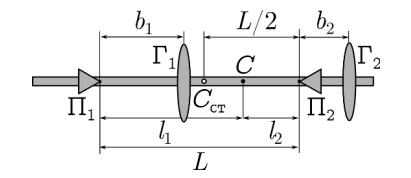
\includegraphics[width=8cm]{рис-1.png}
  \centering
  \caption{Расположение грузов и призм на маятнике.\\С - центр масс маятника, $C_{\text{ст}}$ - центр масс стержня.}
\end{figure}
\normalsize{Запишем уравнение моментов относительно П1:}
\begin{align}
    Ml_1 = m_{\text{ст}}\frac{L}{2}+m_{\text{пр2}}L+m_1b_1+m_2(b_2+L)\text{,}
\end{align}
где $M = m_{\text{ст}}+m_{\text{пр1}}+m_{\text{пр2}}+m_1+m_2$ - полная масса маятника.

В данном методе расчета моменты инерции вычисляются относительно точки подвеса маятника П2. Найдем $b_1 \text{ и } b_2$.\\
\begin{itemize}
    \item{момент инерции тонкого стержня длиной $l_{\text{ст}}$ c призмами:}
        $$I_{\text{ст}} = m_{\text{ст}}\left(\frac{{l_{\text{ст}}}^2}{12}+\left({\frac{L}{2}}^2\right)\right)+m_{\text{пр2}}L^2\text{,}$$
    \item{момент инерции гурзов на стержне:}
        $$I_{\text{гр}} = m_1(L-b_1)^2+m_2{b_2}^2\text{,}$$,
    \item{суммарный момент инерции всего маятника:}
        $$I_{\text{п2}} = MLl_2 = I_{\text{ст}}+I_{\text{гр}}\text{,}$$.
\end{itemize}
\textbf{Измеренные данные:}
\begin{table}[H]
    \centering
    \begin{tabular}{|c|c|c|c|c|c|c|}
        \hline
        $m_i$ & $m_{\text{ст}}$ & $m_{\text{пр1}}$ & $m_{\text{пр2}}$ & $m_1$ & $m_2$ & $M$ \\ \hline
        $m$, гр & 868.2 & 78.3 & 79.6 & 1483.8 & 1508 & 4017.9\\ \hline
        $l_i$ & $l_{\text{ст}}$ & $L$ & $l_2$ & $l_1$ & - & -\\ \hline
        $l$, см & 100 & 52 & 13 & 39 & - & - \\ \hline
    \end{tabular}
    \caption{Массы и длины установки}
    \label{tab:my_labe_1}
\end{table}

\begin{figure}[ht]
  \centering
  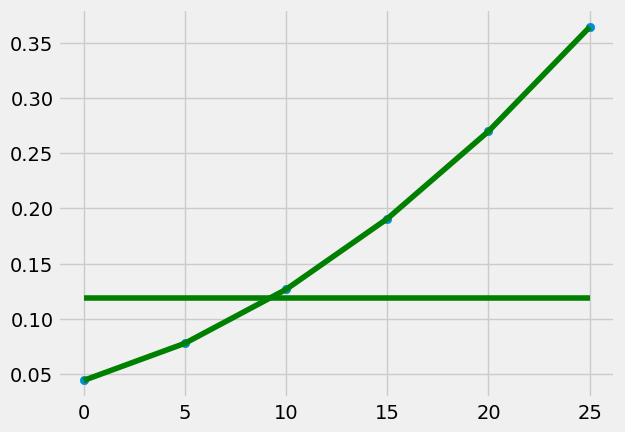
\includegraphics[width=8cm]{рис-2.png}
  \centering
  \caption{График зависимости $I_{\text{гр}}(b_2)$}
\end{figure}
Из графика получаем значения для $b_1 = 9\text{см} \text{ и } b_2 = 25.6\text{см}$.
\section*{Рузультаты измерений и обработка данных} \\[6pt]
\begin{table}[H]
    \centering
    \begin{tabular}{|c|c|c|c|c|}
        \hline
        $20T_1$, с & 29.01 & 29.01 & 29.01 & 29.01\\ \hline
        $20T_2$, с & 29.04 & 29.03 & 29.03 & 29.03\\ \hline
    \end{tabular}
    \caption{Время колебаний маятника в разных точках подвеса П1 И П2(20 периодов)}
    \label{tab:my_labe_2}
\end{table}

\begin{table}[H]
    \centering
    \begin{tabular}{|c|c|c|c|c|c|c|}
        \hline
        $T_1(T)$, с & $T_2(T+\Delta T)$, c & \sigma_T, с & \Delta T, с & \sigma_l, см & \Delta l, см & \beta\\ \hline

        1.4505 & 1.4515 & 0.001 & 0.001 & 0.5 & 26 & 0.5\\ \hline
    \end{tabular}
    \caption{Результаты измерений и погрешности}
    \label{tab:my_labe_3}
\end{table}

\newpage

\subsection*{Определение погрешностей}
Из формул (4)-(6):
\begin{equation}
    g = g_0\frac{\lambda - 1}{\lambda - (1+\varepsilon_t)^2} \approx g_0(1+2\beta \varepsilon_t)\text{,}\\
\end{equation}
\text{где $\varepsilon_t = \frac{\Delta T}{T}$, $\beta = \frac{1}{\lambda - 1} = \frac{l_2}{l_1 - l_2}$.}\\
\text{Tогда:}\\
\begin{equation}
    \varepsilon_{g_0} &= \sqrt{{\left(\frac{\sigma_L}{L}\right)}^2+{\left(\frac{2\sigma_T}{T}\right)}^2}
\end{equation}
\begin{equation}
    \Delta g &\approx \frac{2l_2}{l_1-l_2}\frac{\Delta T}{T}g_0
\end{equation}
\begin{equation}
    \varepsilon_g &\approx \sqrt{{\left(\frac{\sigma_L}{L}\right)}^2 + 4{\left(\frac{\sigma_T}{T}\right)}^2 + 8{\left(\beta\frac{\sigma_T}{T}\right)}^2 +8{\left(\beta\frac{\Delta T}{T}\frac{\sigma_l}{\Delta l}\right)}^2}
\end{equation}

$\varepsilon_g = 0.97\%$

Получаем $g = (9.76 \pm 0.09)$ м/c^2
\section*{Результаты и выводы}
\normalsize{В результате работы для величины $g$ ускорения свободного падения получилось значение $g = (9.76 \pm 0.09)$ м/c^2.Табличная величина
для Москвы: $9.81$ м/с^2. И оно входит в ворота погрешности. Оценим точность метода.Из формулы (9) видно, что погрешность зависит от 
точности измерения трех величин - времени колебаний, отличием времени колебаний в разныз точках подвеса
и расстояния между призмами. Суммарная погрешность измерения времени $\sigma_T = 0.001$ c, тогда $\varepsilon_t = 0.01\%$
Для $T_1$ и $T_2$ погрешность так же составила порадка $0.0001\%$. Тогда точность определения ускорения свободного падения
зависит от точности измерения длины ($\varepsilon_l = 1\%$) порядка одного процента. Тогда погрешность определения $g$ составляет порядка
$1\%$. Так что этот метод можно назвать достаточно точным.}









 
